
\documentclass{article}
\title{[Magic Stones] Report for Experiment 2 - Reverse Order}
\author{Bonan Zhao (b.zhao@ed.ac.uk)}

% Text formats: margin, font, spacing
\usepackage[margin=0.8in]{geometry}
\usepackage{charter}
\renewcommand{\baselinestretch}{1.3}

% Graphics
\usepackage{graphicx}
\usepackage{subcaption}
\graphicspath{{../figs/}}

\usepackage{amsmath}

\begin{document}
\maketitle


\begin{itemize}
  \item Age: min 23, max 65, mean 39.0563, sd 11.161 
  \item Gender: female 28 (39.44\%), male 42 (59.15\%), noresponse 1.
  %\item Task duration (minutes): min 2.2068, max 10.0976, mean 4.8756, sd 1.8663
  %\item Self-report difficulty: min 0, max 10, mean 4.6557, sd 3.1564
\end{itemize}

\begin{table}[h!]
  \centering
  \begin{tabular}{c|l|c|c|c}
  Condition & Description & Count & Task dur. mean (min.) & S-Dfty. mean \\
  \hline
  1 & Agent shape + self color  & 10  & 4.16 & 3.8  \\
  2 & New shape + self color    & 12  & 4.62 & 4.42 \\
  3 & Agent color + self shape  & 9   & 6.22 & 4.11 \\
  4 & New color + self shape    & 7   & 7.27 & 6.29 \\
  5 & Agent color + agent shape & 10  & 5.40 & 5    \\
  6 & Agent color + new shape   & 12  & 4.12 & 3.75 \\
  7 & New color + new shape     & 11  & 6.55 & 5.73 \\
  \hline
  Total    &                       & 71    & & \\
  \end{tabular}
  \caption{Basic stats per condition. S-Dfty.: Self-report difficulty.
  *: Same color + diff shape.}
  \label{table:conditions}
\end{table}

\subsection*{Homogeneity}

Homogeneity is defined as a scaled variance of selection frequency. Homogeneity $H$ for a trial $t_i$ for condition $C$ is calculated by

\[
var(\{\frac{n_{t_i}}{\sum_{i=1}^{15} n_{t_i}} | t_i \in C\})/var(M)
\]
where $M = \{1, \underbrace{0, ..., 0}_{14}, \}$

\begin{table}[h!]
\centering
\begin{tabular}{c|l|l|l}
Condition & Description               & Default & Reverse \\
\hline
01        & Agent shape + self color  & .7469   & .4795   \\
02        & New shape + self color    & .5185   & .4177   \\
03        & Agent color + self shape  & .5710   & .3629   \\
04        & New color + self shape    & .3406   & .4244   \\
05        & Agent color + new shape   & .3662   & .3820   \\
06        & Agent color + agent shape & .6550   & .4500   \\
07        & New color + new shape     & .1981   & .1694  
\end{tabular}
\end{table}

\begin{figure}[h!]
  \centering
  \begin{subfigure}[t]{0.45\textwidth}
    \centering
    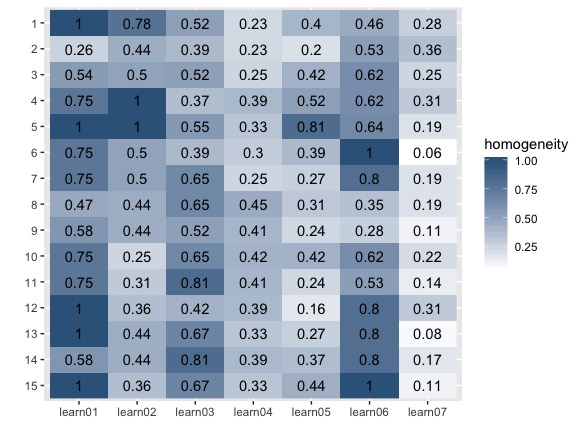
\includegraphics[width=\linewidth]{var_ind} 
    \caption{Individual - default order}
  \end{subfigure}
  \begin{subfigure}[t]{0.45\textwidth}
    \centering
    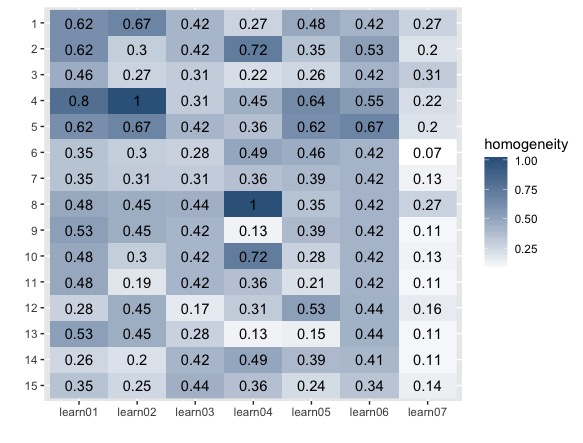
\includegraphics[width=\linewidth]{var_rev_ind} 
    \caption{Individual - reverse order}
  \end{subfigure}

  \begin{subfigure}[t]{0.45\textwidth}
    \centering
    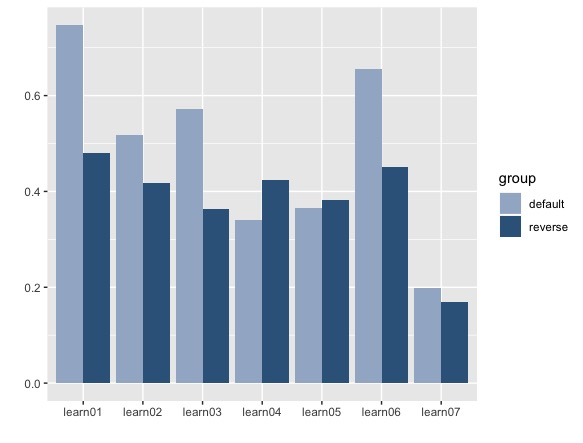
\includegraphics[width=\linewidth]{var_cond} 
    \caption{Aggregated by conditions}
  \end{subfigure}
  \begin{subfigure}[t]{0.45\textwidth}
    \centering
    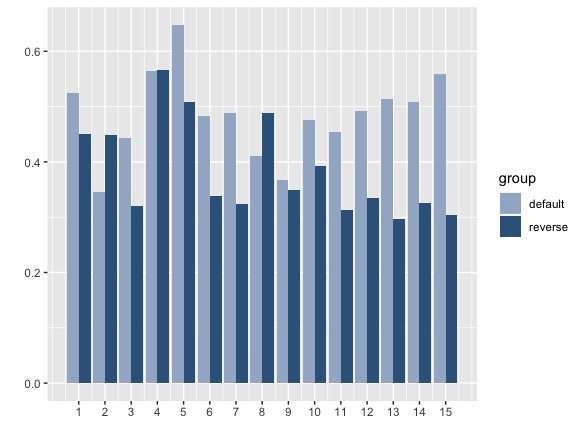
\includegraphics[width=\linewidth]{var_t} 
    \caption{Aggregated by tasks}
  \end{subfigure}
  \caption{Homogeneity.}
  \label{fig:var}
\end{figure}



% Raw participant data
\subsection*{Raw data}

\begin{figure}[h!]
  \begin{subfigure}[t]{0.32\textwidth}
  	\centering
  	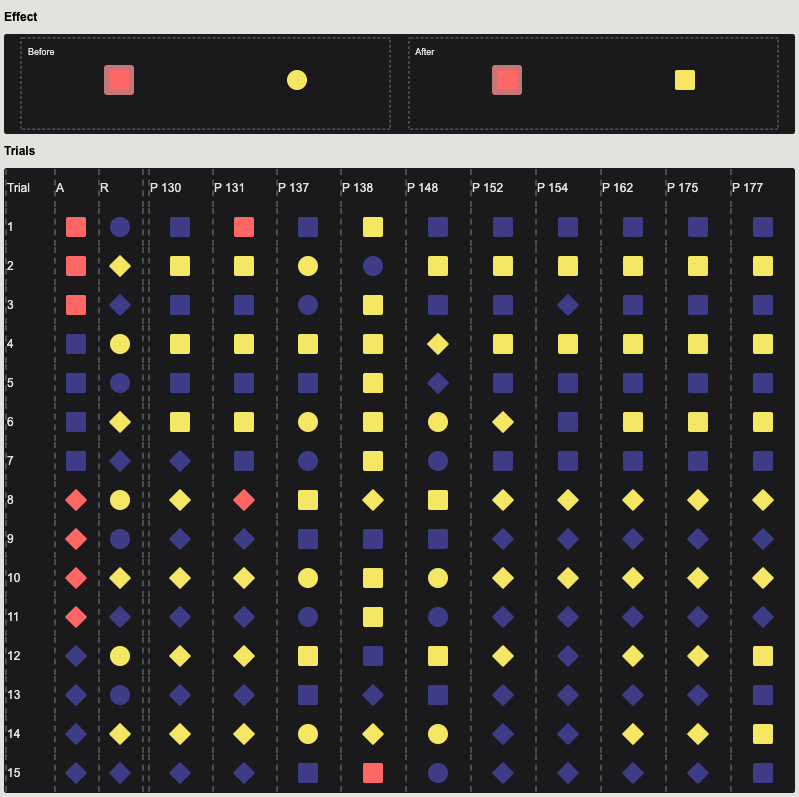
\includegraphics[width=\linewidth]{rev_01} 
  	\caption{Agent shape + Self color} \label{fig:learn01}
  \end{subfigure}
  \begin{subfigure}[t]{0.32\textwidth}
  	\centering
  	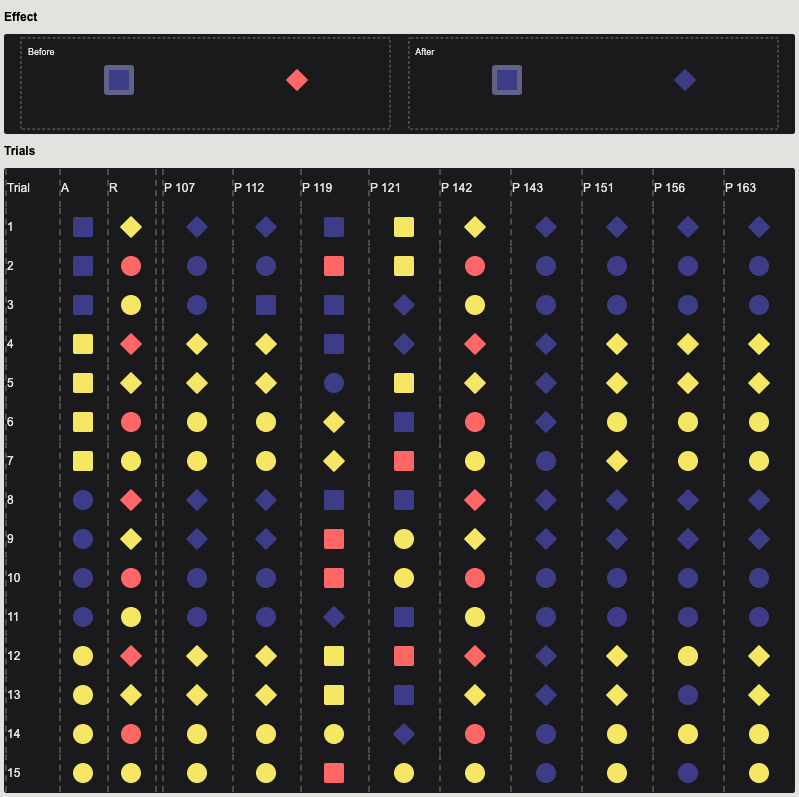
\includegraphics[width=\linewidth]{rev_03} 
  	\caption{Agent color + Self shape} \label{fig:learn03}
  \end{subfigure}

  \begin{subfigure}[t]{0.32\textwidth}
  	\centering
  	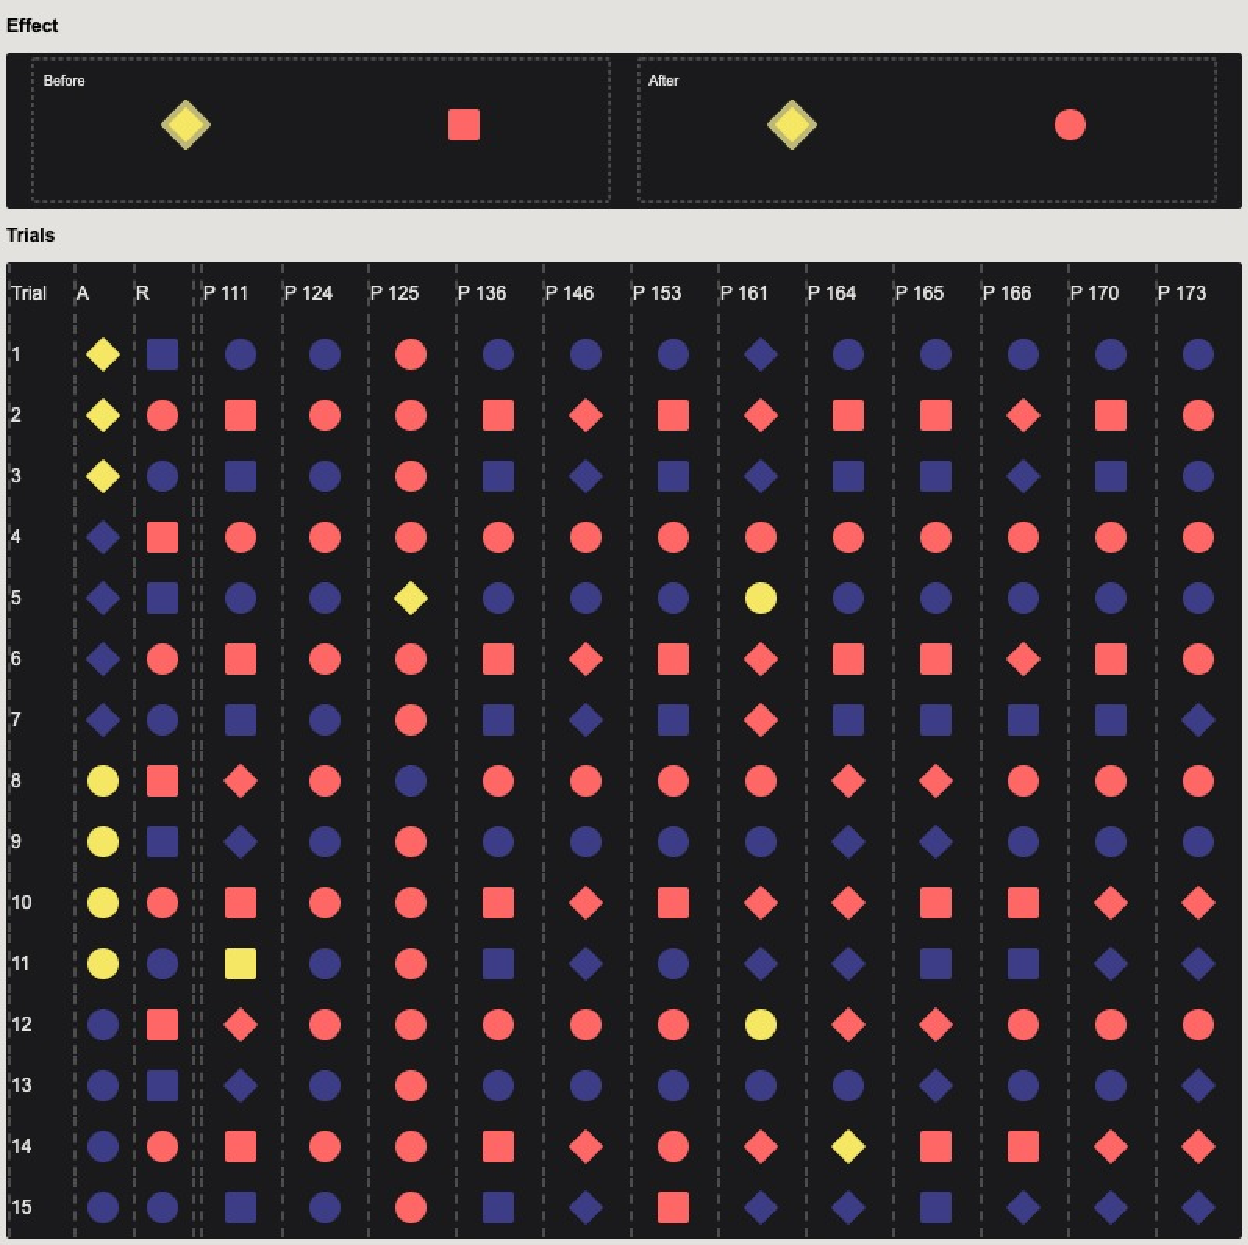
\includegraphics[width=\linewidth]{rev_02} 
  	\caption{New shape + self color} \label{fig:learn02}
  \end{subfigure}
  \begin{subfigure}[t]{0.32\textwidth}
  	\centering
  	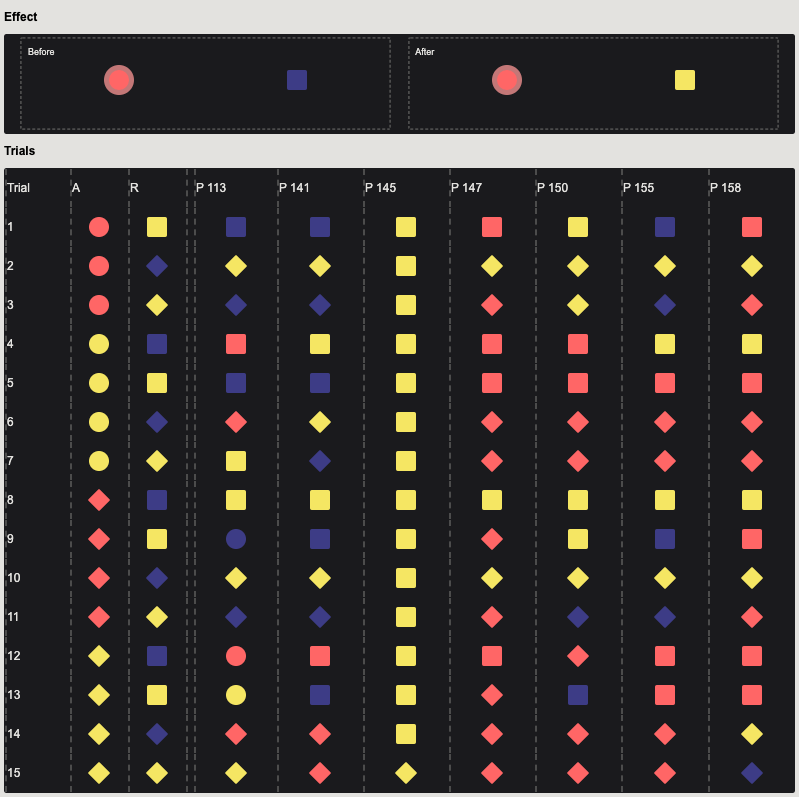
\includegraphics[width=\linewidth]{rev_04} 
  	\caption{New color + self shape} \label{fig:learn04}
  \end{subfigure}

  \begin{subfigure}[t]{0.32\textwidth}
    \centering
    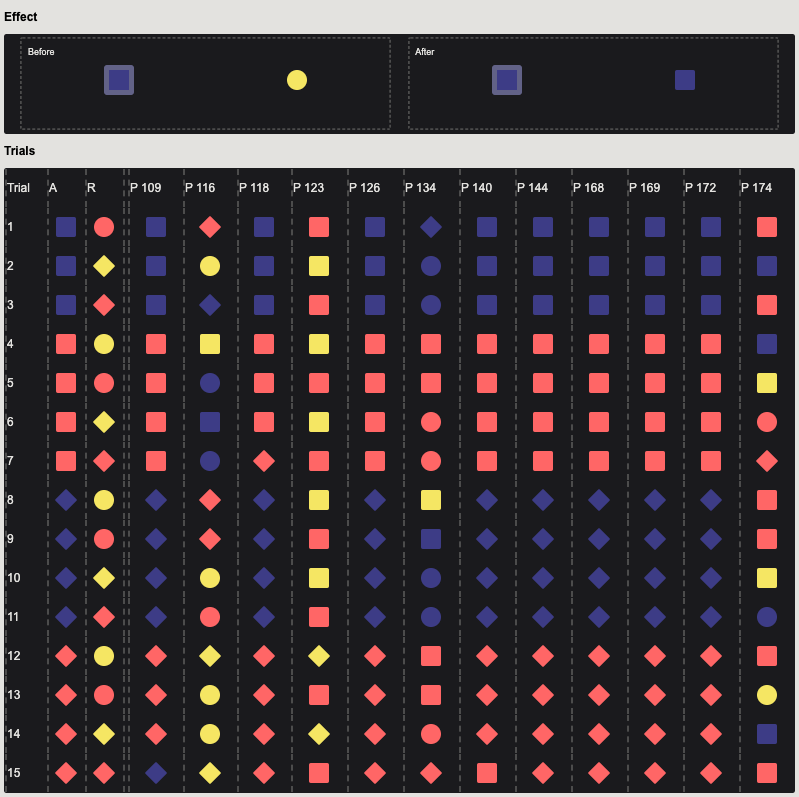
\includegraphics[width=\linewidth]{rev_06} 
    \caption{Agent color + Agent shape} \label{fig:learn06}
  \end{subfigure}
  \begin{subfigure}[t]{0.32\textwidth}
    \centering
    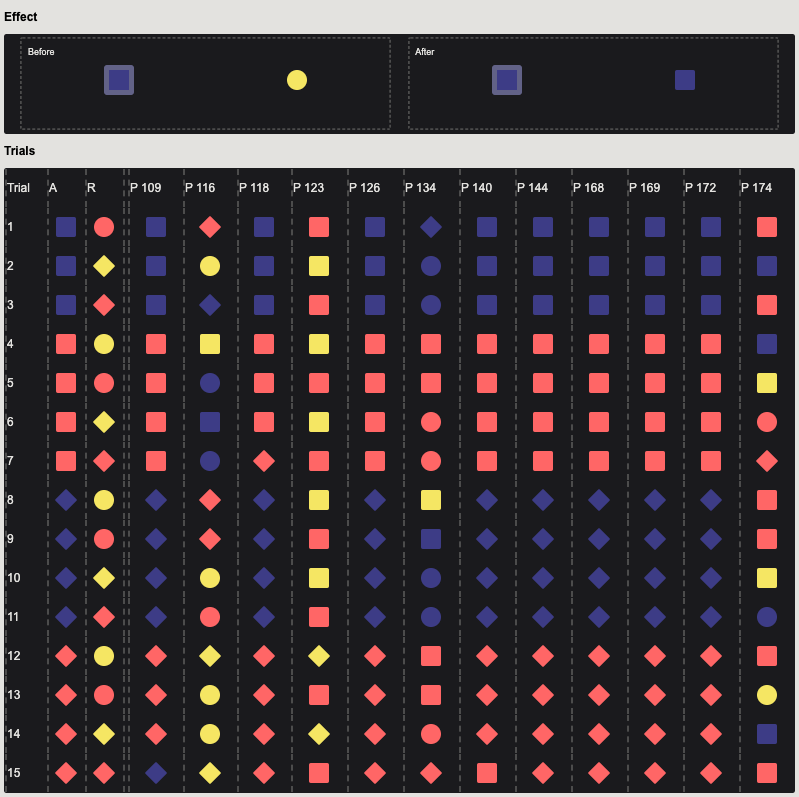
\includegraphics[width=\linewidth]{rev_06} 
    \caption{Agent color + new shape} \label{fig:learn06}
  \end{subfigure}
  \begin{subfigure}[t]{0.32\textwidth}
    \centering
    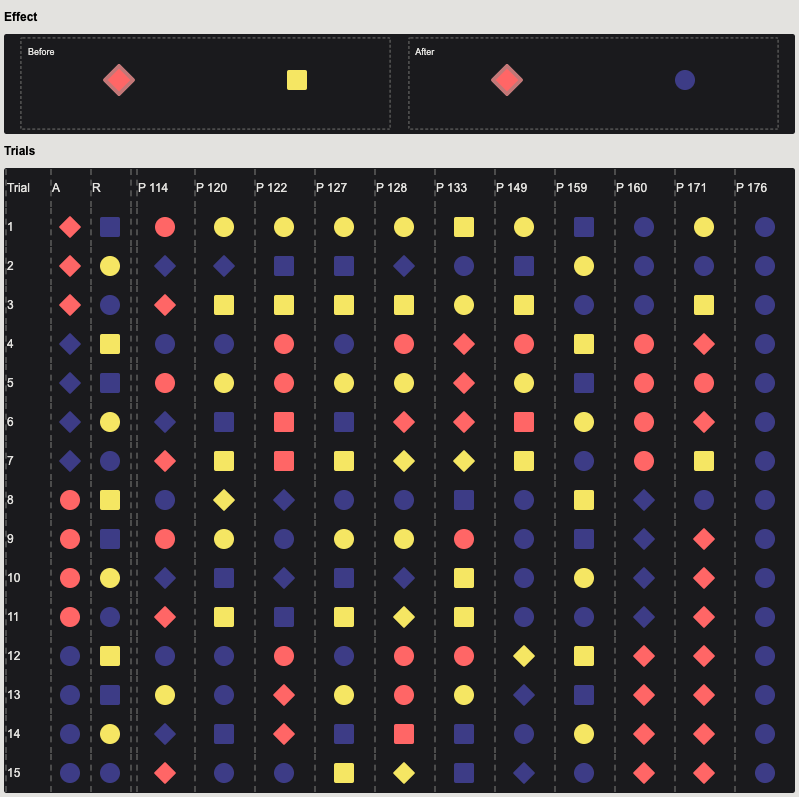
\includegraphics[width=\linewidth]{rev_07} 
    \caption{New color + new shape} \label{fig:learn07}
  \end{subfigure}
  \caption{Each figure is for one learning condition. 
  Each learning condition has 15 trials (15 rows).}
\end{figure}


\end{document}


